\chapter{Arquitectura del Chatbot}
\label{cap:arquitectura}

Los sistemas de análisis automático de texto tienen como objetivo entender la información no estructurada hablada por los humanos y convertirla en información estructurada como podría ser un resumen del contenido o la clasificación de un documento por temática.

En el caso que nos ocupa, el objetivo del chatbot es conseguir esta información estructurada a partir de la mayor cantidad de recuerdos posibles para ayudar a los terapeutas a construir la historia de vida de un paciente que es mucho más complicada de tratar en bruto. Antes de estructurarla, primero hay que conseguir la información a través de las conversaciones con la persona. De esto se encargará uno de los módulos del bot (detallado en la sección \ref{rep_preguntas}) que planteará todo tipo de preguntas para recopilar el máximo número de recuerdos. Estas preguntas se extraen de una base de datos de tipo MongoDB y se eligen de forma ordenada.

Las respuestas que da el usuario también se almacenan en Mongo, pero previamente se procesan. El análisis de estas respuestas se va a realizar en varios sentidos, por un lado, se clasificarán los recuerdos en etapas de vida, para estructurar la información lo máximo posible. Por otro lado, se determinará si el texto contiene connotaciones positivas o negativas, de tal forma que en la terapia se puedan evitar los recuerdos negativos que pueden agravar la situación del paciente. Estos dos procesamientos mencionados pertenecen al módulo de clasificación de recuerdos explicado con más detalle en la sección \ref{clasificacion_rec}. Por último, se utilizará el procesamiento del lenguaje natural mediante el análisis morfológico de las palabras para comprender lo que quiere decir el paciente y poder generar la siguiente pregunta más acertada y relacionada con la temática que se está tratando. Este último apartado compondrá el módulo de procesamiento del texto para encadenar preguntas y respuestas descrito en la sección \ref{procesamiento}.

En resumen, para el funcionamiento íntegro del chatbot, deben estar presentes tres módulos: el módulo de las preguntas, el módulo de la clasificación de recuerdos y el módulo de elección de la mejor siguiente pregunta. Se explican a continuación, uno por sección.

\section {Repertorio de preguntas} \label{rep_preguntas}

El Chatbot que se ha desarrollado no funciona como la mayoría de agentes que se han creado a lo largo de los últimos años. Siri por ejemplo es uno de ellos y funciona de tal manera que es el usuario quien conduce la conversación haciendo preguntas o peticiones. Este programa se diferencia de los demás porque, por el contrario, es el bot quien dirige la conversación planteándole preguntas al usuario. 

El sistema funciona realizando una primera pregunta y, a continuación, por cada respuesta que dé el usuario se formula otra pregunta. Esta pregunta estará lo más relacionada posible con la contestación previamente recibida, módulo que se explicará en la sección \ref{procesamiento}. 

El repertorio de preguntas se extrae de la base de datos de MongoDB. Esta colección de cuestiones se ha ido formando a lo largo del TFG mediante la reformulación de preguntas sacadas de documentos de terapia ocupacional ofrecidos por expertos terapeutas del proyecto CANTOR. Es decir, no se han cogido directamente de estos documentos con entrevistas, sino que se han ido redactando y adaptando según las necesidades que iban surgiendo para el Chatbot. 

\section{Clasificación de los recuerdos} \label{clasificacion_rec}

Tal y como se explica en la introducción de este capítulo, este módulo de clasificación tiene dos componentes, el que analiza el sentimiento del texto y distingue entre recuerdos positivos y negativos y, el que categoriza por etapas de vida. Ambos están fundamentados en base a la misma idea y utilizan el mismo método de clasificación automática basado en etiquetas.

Para poder llevar a cabo la distinción de categorías dentro de un texto se ha utilizado la librería \textit{Spacy} de Python que cuenta con un componente llamado ``TextCategorizer''\footnote{https://spacy.io/api/textcategorizer}. Este componente permite entrenar un modelo capaz de predecir las categorías o etiquetas que se quieran identificar de un texto como en este caso, frases positivas o frases negativas. Se probaron otras tecnologías y librerías de Python para conseguir un resultado parecido. Dos de las librerías consideradas fueron ``NLTK'' y ``Chatterbot''. Pero, finalmente se eligió \textit{Spacy} por su versatilidad, su amplia oferta de funcionalidades y por la facilidad con la que se pueden tokenizar textos. De cara a la evolución del trabajo, prevista en un principio, se trataba de la mejor herramienta para poder ampliar el chatbot gracias a sus componentes destinados al procesamiento del lenguaje natural. 

Una vez elegida, se probó primero la herramienta ``TextCategorizer'' para la clasificación de los recuerdos en positivos y negativos. Por ello, se empezará a explicar haciendo referencia únicamente al análisis de sentimientos. Más adelante en esta sección (apartado \ref{clasificacion_etapasvida}) se explicará cómo se adaptó para el módulo de clasificación en etapas. 

\textit{Spacy} proporciona algoritmos de aprendizaje automático que observan unos datos facilitados y construye a partir de ellos un modelo capaz de clasificar gracias a la estadística. Estos algoritmos son los que interesan a la hora de construir el categorizador de textos. Como guía de uso de estas herramientas, se ha utilizado el artículo \textit{How to Train Text Classification Model in spaCy}\footnote{https://www.machinelearningplus.com/nlp/custom-text-classification-spacy/}.

Los datos iniciales proporcionados para entrenar al modelo suelen proceder de datasets muy grandes para que el modelo sea lo más preciso posible. En este caso, el objetivo es diferenciar los recuerdos negativos de los positivos y así tener la primera clasificación que pidieron los terapeutas especializados del proyecto CANTOR. Es por ello que lo interesante es utilizar un conjunto grande de recuerdos tanto positivos como negativos. Antes de probar con recuerdos se probó el funcionamiento del  ``TextCategorizer'' con un dataset muy grande de reseñas de moda que se ponía como ejemplo en el artículo del que se hablaba anteriormente. Con ello se comprobó la precisión de clasificación y se pasó a adaptarlo a la situación de este TFG. Al no encontrar ningún dataset de recuerdos por ningún lado, se ha usado una batería relativamente pequeña (comparado con el tamaño habitual de entrenamiento) de recuerdos positivos encontrados entre los archivos del TFG de \cite{lcastilla}. No se cogieron estos textos directamente, sino que se acortaron y adaptaron para formar recuerdos más concretos. También había que incluir recuerdos negativos y para ello se han usado frases negativas inventadas, pensadas para entrenar el modelo de la mejor manera posible. Concretamente, se consiguió reunir una cantidad de 32 recuerdos negativos frente a 140 positivos. A continuación se muestran ejemplos de algunos de los textos:

Positivos:
\begin{itemize}
	\item ``El año pasado mis abuelos celebraron 60 años de casados''
	\item ``Cuando era niña, disfrutaba de las bandas sonoras de las películas de Disney''
\end{itemize}

Negativos:
\begin{itemize}
	\item ``A los 14 años mi padre se murió de cáncer''
	\item ``No me llevaba bien con mi hermano Jorge y todavía hoy no nos llevamos bien.''
\end{itemize}

En cuanto al desarrollo del código, el proceso de categorización de recuerdos funciona siguiendo una serie de pasos. En la figura \ref{fig:flujo_cat} se encuentra el diagrama de flujo del clasificador con cada uno de los pasos que sigue para entrenar un modelo y poder, así, predecir las categorías. 

\begin{figure}
	\centering
	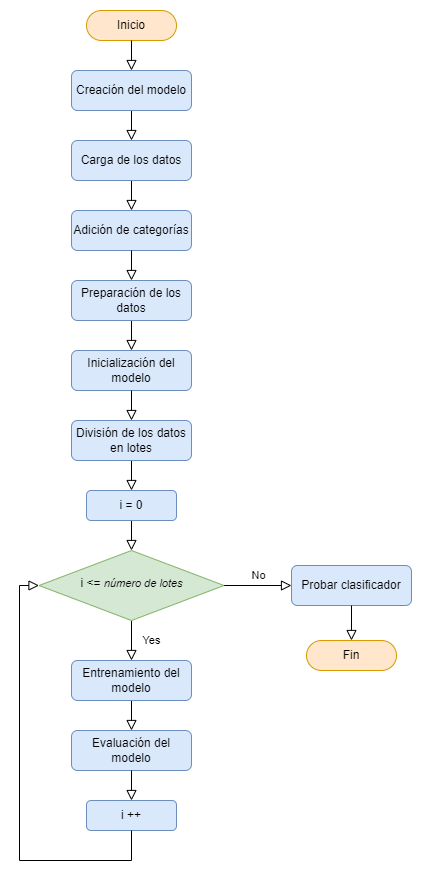
\includegraphics[scale=0.7]{Imagenes/Vectorial/diagrama_flujo_categorizador}
	\caption{Diagrama de flujo del categorizador}
	\label{fig:flujo_cat}
\end{figure}

En primer lugar, se define el modelo. Puede crearse vacío o se puede cargar directamente un modelo pre-entrenado con una serie de componentes. Un componente es una función que se aplica a un texto y que lo devuelve procesado de alguna forma. Por ejemplo, el componente ``NER'', más reconocido como \textit{Named Entity Recognizer}, reconoce entidades dentro del texto como nombres de personas, fechas o lugares. Para nuestro caso en concreto, se crea un modelo en blanco y se le añade el componente ``TextCategorizer'' (textcat). Un modelo en blanco es un modelo que no tiene ningún componente de spaCy definido, es decir, el texto que se quiera procesar no será analizado por ninguna cadena de funciones. El texto procesado que devuelva el modelo se mantiene intacto. Si se hubiese cogido un modelo pre-entrenado como es ``es\_core\_news\_sm'', se habría añadido el componente de clasificación de textos por encima del resto de componentes. Es decir, se sumaría al trabajo de los procesos que analizan el texto. En el caso de ``es\_core\_news\_sm'' está compuesto por una serie de funciones (componentes) que se ejecutan en orden. Algunas de ellas son:

\begin{itemize}
	\item ``tok2vec'': transforma los tokens en vectores (array de valores numéricos) para que la máquina pueda entender una secuencia de caracteres.
	\item ``morphologizer'': analiza morfológicamente los tokens
	\item ``lemmatizer'': halla el lema de las palabras
	\item ``ner'': reconoce entidades, explicado anteriormente
\end{itemize}

En este caso, no se necesitaban las funciones que ofrecían los modelos pre-entrenados y por eso se empieza con uno vacío. Al usar el modelo en blanco se empieza con el español de cero, sin nada que analizar. Tras añadir el componente textcat, cualquier texto a tratar por el modelo, automáticamente, pasará por el proceso de clasificación que le indiquemos. Para que textcat funcione como categorizador de recuerdos, se le añade a nuestro nuevo componente dos etiquetas, NEGATIVO y POSITIVO, que definirán cuánto de negativo es un recuerdo y cuánto de positivo. Para seguir configurando esta función, es necesario cargar los datos iniciales, aquellos recuerdos seleccionados anteriormente que serán los que entrenen al modelo. Esta información se prepara antes de ser procesada para que el clasificador la entienda. Es decir, los datos se adecuan al formato que entiende el modelo siendo éste una lista de tuplas (texto, categoría). Por ejemplo: \\

\begin{verbatim}
	(El año pasado mis abuelos celebraron 60 años de casados, 
			{'cats': {'POSITIVO': True, 'NEGATIVO': False}}) 
\end{verbatim}


El modelo reservará un porcentaje de esta batería de recuerdos (\% que previamente se define) para la evaluación de las predicciones, es decir, para analizar cómo de bien predice el modelo tras entrenarlo. 

Ya está todo preparado para comenzar a entrenar el modelo, se dividen los casos de entrenamiento en lotes que se analizan y evalúan un número definido de iteraciones para asegurar que el entrenamiento es lo más preciso posible. Se trata de unos valores que pueden variar según la necesidad de entrenamiento que surja. Es importante no superar un número de repeticiones para que el algoritmo también sea óptimo, es decir, el número de vueltas debe permitir que el entrenamiento sea eficaz pero también que sea eficiente. No permitir que el costo del algoritmo sea demasiado grande, esto depende de la cantidad de datos con los que se vaya a entrenar el modelo. En este caso, como el volumen de datos iniciales es pequeño, se apuesta por ocho iteraciones. El modelo se entrena utilizando una función de \textit{Spacy} que lo analiza y actualiza en cada repetición con lo nuevo que ha aprendido: la función update\footnote{https://spacy.io/api/textcategorizer\#update}. Funciona de la siguiente forma: 
\begin{enumerate}
	\item Se inicializan los parámetros del modelo de forma aleatoria.
	\item Se predice el primer lote de ejemplos con los parámetros que se han fijado.
	\item Se revisan estas predicciones comparándolas con las etiquetas correctas.
	\item Se decide cómo cambiar los parámetros actuales para obtener mejores predicciones en las próximas veces.
	\item Se hace la pequeña corrección de los parámetros.
	\item Vuelta al paso 2 pero con el siguiente lote de ejemplos.
\end{enumerate}
Se repite este bucle de entrenamiento hasta que el modelo deje de mejorar. En la figura \ref{fig:entrenamiento} sacada del manual de \textit{Spacy}\footnote{https://course.spacy.io/es/chapter4} se puede visualizar cómo funciona. 

\begin{figure}[h]
	\centering
	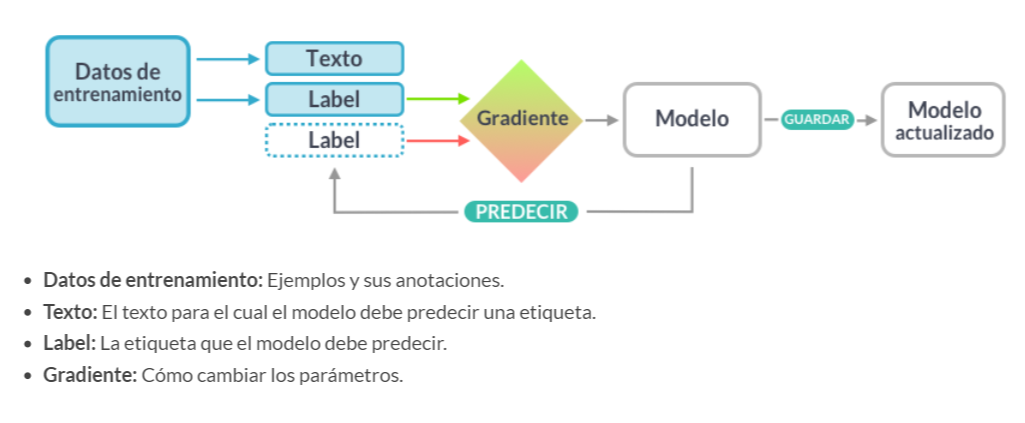
\includegraphics[scale=0.5]{Imagenes/Vectorial/entrenamiento_modelo}
	\caption{Entrenamiento del modelo}
	\label{fig:entrenamiento}
\end{figure}

Además, en cada vuelta, también se realizan una serie de pruebas para comprobar la precisión de las predicciones, se comparan con las etiquetas de referencia para estimar la desviación de la pérdida, es decir, cuánto de alejado se encuentra del valor real. Estas comprobaciones se realizan para asegurarse que el algoritmo está haciendo bien las cosas.

Una vez afinado el modelo mediante el entreno previo, ya se puede poner a prueba. El clasificador sacará la probabilidad entre 0 y 1 de que un texto procesado por spacy sea un recuerdo positivo y la probabilidad de que sea uno negativo de esta forma:

\begin{verbatim}
	Texto analizado: {'POSITIVO': probabilidad entre 0 y 1,
		 'NEGATIVO': probabilidad entre 0 y 1}
\end{verbatim}

Como se trata de dos etiquetas mutuamente excluyentes, la probabilidad de una será la diferencia de la otra. Así, la que mayor probabilidad tenga será la elegida como predicción final. Si la probabilidad de que sea un texto positivo es mayor que la de que sea negativo, el recuerdo será finalmente evaluado como positivo y lo mismo al revés.

En resumen, como se ha explicado, el programa entrena primero al modelo con textos positivos y negativos y luego evalúa el texto que le llega del usuario e identifica si es negativo o positivo. Esto se utilizará como una de las categorías que se le asignan a cada respuesta recibida y que se mete en una base de datos Mongo junto a la respuesta que haya dado el usuario al chatbot. Este análisis de sentimiento también servirá para identificar temáticas dolorosas para el interrogado que no deberían ser usadas en las terapias.

Más adelante en el proyecto, se observó que, al analizar el sentimiento de la frase, había recuerdos o simplemente, datos que no encajaban en ninguna de las dos categorías de positivo y negativo. Las emociones neutras son aquellas que no son desagradables ni agradables, es decir, ni negativas ni positivas. Es por esto que se probó a añadir una nueva categoría para los datos neutro como por ejemplo, indicar tu edad, explicar dónde vivías en cierto momento de tu vida, etc. No suponía un gran esfuerzo porque el programa estaba pensado para poder añadir todas las categorías que se considerasen. Sin embargo, a niveles prácticos, se pudo comprobar que no funcionaba igual de bien que la clasificación binaria. El nivel de entrenamiento que necesitaría el modelo para poder distinguir también las frases neutras es mucho mayor, es decir, se necesitarían muchos más casos, ejemplos, para que el modelo aprendiese de ellos. En este caso, solo se añadieron alrededor de 40 recuerdos neutros, de nuevo inventados, por la falta de recursos encontrados en Internet que no proporcionaba ningún dataset parecido al que se buscaba. En la siguiente sección de pruebas se podrá comprobar la diferencia entre meter la categoría neutra y no meterla. 

\subsection{Pruebas del análisis de sentimiento}

Para comprobar la precisión y el correcto funcionamiento del módulo de análisis de sentimiento, se hicieron una serie de pruebas que corroboraron que la clasificación en recuerdos negativos y positivos funcionaba relativamente bien pero que podría mejorarse metiendo muchos más casos de entrenamiento para afinar el modelo. A continuación se muestran algunos ejemplos de frases que se han analizado con el categorizador de textos y las conclusiones que se han sacado. Entre llaves se muestra la probabilidad sobre 1 de que la frase sea positiva y la probabilidad sobre 1 de que sea negativa. Entre corchetes se muestra la categoría a la que pertenece la frase por tener la mayor probabilidad las dos:

\begin{itemize}
	\item ``Mi abuela se murió en 1998''
	\begin{verbatim}
		{'POSITIVO': 0.09926079958677292, 'NEGATIVO': 0.9007392525672913}
		['negativo']
	\end{verbatim}
	\item ``Mi mejor recuerdo es el del nacimiento de mi hijo''
	\begin{verbatim}
		{'POSITIVO': 0.992607593536377, 'NEGATIVO': 0.007392475381493568}
		['positivo']
	\end{verbatim}
	\item ``Tengo 23 años''
	\begin{verbatim}
		{'POSITIVO': 0.9999983310699463, 'NEGATIVO': 1.6568293403906864e-06}
		['positivo']
	\end{verbatim}
	\item ``Me dolió muchísimo cuando me rompí una pierna''
	\begin{verbatim}
		{'POSITIVO': 2.0322097043390386e-05, 'NEGATIVO': 0.9999797344207764}
		['negativo']
	\end{verbatim}
	\item ``Mi hermano y yo nos pasábamos las tardes haciendo puzles''
	\begin{verbatim}
			{'POSITIVO': 0.9681606888771057, 'NEGATIVO': 0.031839337199926376}
		['positivo']
	\end{verbatim}
	\item ``Durante la infancia estuvimos viviendo en Moratalaz''
	\begin{verbatim}
		{'POSITIVO': 0.9882893562316895, 'NEGATIVO': 0.011710633523762226}
		['positivo']
	\end{verbatim}
	\item ``Mi pareja sufrió depresión después del parto''
	\begin{verbatim}
		{'POSITIVO': 0.07562904059886932, 'NEGATIVO': 0.9243709444999695}
		['negativo']
	\end{verbatim}

\end{itemize}

Por otro lado, también se probó cómo funcionaba el programa añadiendo la clasificación de neutro. Podemos comparar así ambas formas de clasificación y comprobar que, efectivamente, funciona mejor el binario. De nuevo, entre llaves se muestra la probabilidad sobre 1 de que la frase sea positiva, la probabilidad sobre 1 de que sea negativa y la probabilidad sobre 1 de que sea neutra. Entre corchetes se muestra la categoría a la que pertenece la frase por tener la mayor probabilidad de todas:

\begin{itemize}
	\item ``Mi abuela se murió en 1998''
	\begin{verbatim}
		{'POSITIVO': 0.000133998051751405, 'NEGATIVO': 0.00039583168108947575,
			'NEUTRO': 0.9994701743125916}
		['neutro']
	\end{verbatim}
	\item ``Mi mejor recuerdo es el del nacimiento de mi hijo''
	\begin{verbatim}
		{'POSITIVO': 0.0003367967437952757, 'NEGATIVO': 0.9894788861274719, 
			'NEUTRO': 0.010184396989643574}
		['negativo']
	\end{verbatim}
	\item ``Tengo 23 años''
	\begin{verbatim}
		{'POSITIVO': 0.016445694491267204, 'NEGATIVO': 0.0031412760727107525, 
			'NEUTRO': 0.980413019657135}
		['neutro']
	\end{verbatim}
	\item ``Me dolió muchísimo cuando me rompí una pierna''
	\begin{verbatim}
		{'POSITIVO': 0.0006958534941077232, 'NEGATIVO': 0.9989858269691467, 
			'NEUTRO': 0.0003183614171575755}
		['negativo']
	\end{verbatim}
	\item ``Mi hermano y yo nos pasábamos las tardes haciendo puzles''
	\begin{verbatim}
		{'POSITIVO': 2.354631942580454e-05, 'NEGATIVO': 0.9972598552703857, 
			'NEUTRO': 0.0027166458312422037}
		['negativo']
	\end{verbatim}
	\item ``Durante la infancia estuvimos viviendo en Moratalaz''
	\begin{verbatim}
		{'POSITIVO': 0.051713500171899796, 'NEGATIVO': 0.9064642786979675, 
			'NEUTRO': 0.041822321712970734}
		['negativo']
	\end{verbatim}
	\item ``Mi pareja sufrió depresión después del parto''
	\begin{verbatim}
		{'POSITIVO': 2.2260337573243305e-05, 'NEGATIVO': 0.9954761862754822, 
			'NEUTRO': 0.004501543939113617}
		['negativo']
	\end{verbatim}
	
\end{itemize}

En esta sección de pruebas se puede comprobar que algo no debe estar funcionando del todo bien y que el problema de las predicciones puede estar en las dimensiones del dataset que se le proporciona al modelo. Sin embargo, faltaron pruebas para comprobar que esa era la razón. Aun así, faltos de un dataset grande de recuerdos para el análisis de sentimientos se buscó uno que no fuese de recuerdos como tal pero que sí podría servir para hacer una buena predicción de negativos y positivos. Se encontró un dataset\footnote{https://www.kaggle.com/datasets/luisdiegofv97/imdb-dataset-of-50k-movie-reviews-spanish} en español de 50,000 reseñas de IMBD de películas con un sentimiento positivo o negativo adjunto (no se encuentra ninguno que incluya el neutro). Probando el clasificador cargando esta colección de datos al modelo, se observan los siguientes resultados: 

\begin{itemize}
	\item ``Mi abuela se murió en 1998''
	\begin{verbatim}
		{'POSITIVO': 0.8378736972808838, 'NEGATIVO': 0.16212628781795502}
		['positivo']
	\end{verbatim}
	\item ``Mi mejor recuerdo es el del nacimiento de mi hijo''
	\begin{verbatim}
		{'POSITIVO': 0.9998306035995483, 'NEGATIVO': 0.00016938232874963433}
		['positivo']
	\end{verbatim}
	\item ``Tengo 23 años''
	\begin{verbatim}
		{'POSITIVO': 0.9846466779708862, 'NEGATIVO': 0.015353254973888397}
		['positivo']
	\end{verbatim}
	\item ``Me dolió muchísimo cuando me rompí una pierna''
	\begin{verbatim}
		{'POSITIVO': 0.08775553107261658, 'NEGATIVO': 0.9122444987297058}
		['negativo']
	\end{verbatim}
	\item ``Mi hermano y yo nos pasábamos las tardes haciendo puzles''
	\begin{verbatim}
		{'POSITIVO': 0.999742329120636, 'NEGATIVO': 0.0002577087143436074}
		['positivo']
	\end{verbatim}
	\item ``Durante la infancia estuvimos viviendo en Moratalaz''
	\begin{verbatim}
		{'POSITIVO': 0.9989288449287415, 'NEGATIVO': 0.0010711398208513856}
		['positivo']
	\end{verbatim}
	\item ``Mi pareja sufrió depresión después del parto''
	\begin{verbatim}
		{'POSITIVO': 0.03745762258768082, 'NEGATIVO': 0.9625424146652222}
		['negativo']
	\end{verbatim}
	
\end{itemize}

Podemos observar que acierta todas las frases menos la primera. Se ha probado con más frases relacionadas con la muerte y todas las predice como positivas. En este caso, el entrenamiento parece no haber perfeccionado los resultados, puede ser por la información que proporciona el dataset, que se aleje mucho de lo que pueda surgir de un recuerdo o, por algún fallo en el proceso de entrenamiento.  

En conclusión, lo ideal habría sido tener una colección de datos lo suficientemente grande para entrenar bien al modelo y que estuviese relacionado con los recuerdos y memorias de la vida de personas. Se plantea como trabajo futuro. Por la precisión de los resultados obtenidos finalmente, se optó por el primer entrenamiento, que tiene un dataset pequeño de recuerdos pero funciona relativamente bien, como se ha podido observar en estas pruebas. La aplicación, por ende, funciona con el primer clasificador planteado. 

\subsection{Clasificación en etapas de vida} \label{clasificacion_etapasvida}

Otra de las categorías que se añadirá junto a la respuesta en la base de datos de recuerdos será la de la etapa de vida a la que corresponde el recuerdo. En un principio, había que definir las etapas y se decidió usar de forma orientativa la clasificación que hace el Ministerio de Salud de Colombia\footnote{https://www.minsalud.gov.co/proteccionsocial/Paginas/cicloVida.aspx} porque no se encontraron fuentes fiables españolas que diesen una clasificación tan clara y sensata. Aún así se le hicieron algunas adecuaciones para que se ajustase más a lo que se buscaba y lo que se quería sacar en claro. Además, como en el caso del análisis de sentimiento con el neutro, se decidió desde un principio añadir la clasificación ``Indeterminado'' para aquellos recuerdos que no encajasen en ninguna etapa porque fuesen datos generales. Aquí se veía más claro que había información de los usuarios que era muy general y que por defecto no podía meterse en ninguna otra etapa. Sin embargo, pasaba lo mismo que con el neutro, la clasificación era mucho menos acertada. Más adelante se explicará con más detalle. A continuación se muestra la clasificación inicial que se eligió:

\begin{itemize}
	\item Infancia de 0 a 11 años
	\item Adolescencia de 12 a 17 años
	\item Juventud de 18 a 26 años
	\item Etapa adulta de 27 a 59 años
	\item Vejez de 60 años o más
	\item Indeterminado para aquellos textos en los que no se pueda distinguir la etapa
\end{itemize}

Una vez elegidos los periodos de tiempo en los que se divide la vida de las personas, el objetivo era clasificar recuerdos, dados en forma de respuesta a una pregunta, según la etapa de la vida a la que pertenecía el recuerdo de la persona interrogada. Para ello, también se ha utilizado la misma tecnología que para el análisis de sentimientos. Además de entrenarse en recuerdos positivos y negativos, ahora el modelo se entrena para distinguir etapas vitales en las que ocurren los recuerdos para así, de cara a la elaboración de un libro de vida, toda la información esté bien estructurada en periodos de tiempo. 

Como se explicaba al principio, la clasificación que se eligió inicialmente no resultó dar buenos resultados. El nivel de entrenamiento que necesitaría el modelo para poder distinguir también los recuerdos que no encajan en ninguna de las etapas anteriores es mucho mayor. Además, resultaba muy ambigua la etapa indeterminada porque los recuerdos que se meten en esa clasificación no tienen relación entre ellos para el modelo, no puede aprender de similitudes porque cada recuerdo es muy distinto y muy general. Algo parecido pasaba con la etapa de la adolescencia, no se aprecia bien en los ejemplos la diferencia entre la etapa de la adolescencia y la de la juventud porque no existen ejemplos que hagan una buena distinción entre la una y la otra ya que son muy parecidos los sucesos que podrían ocurrir en una y en la otra. Es por eso que se ha decidido quitar ambas etapas y ponérselo mucho más fácil al modelo para que pueda reconocer bien los recuerdos y no confundirse tan fácilmente. En la sección de pruebas se ve claramente la diferencia entre ambos casos. Finalmente, se ha elegido una  clasificación muy clara según los hechos que suelen pasar en la vida de las personas en las distintas etapas y para los que cada etapa tiene ejemplos precisos y nada ambiguos. Se trata además de una clasificación que se acerca más a lo que los terapeutas están acostumbrados en sus terapias. Se hace la siguiente división:

\begin{itemize}
	\item Infancia de 0 a 12 años
	\item Juventud de 13 a 26 años
	\item Etapa adulta de 27 a 59 años
	\item Vejez de 60 años o más
\end{itemize}


\subsubsection{Pruebas}

Se comprueba la precisión y el correcto funcionamiento del módulo de clasificación en etapas de vida, se hicieron una serie de pruebas que indicaron que la clasificación funcionaba relativamente bien pero que podría mejorarse metiendo muchos más casos de entrenamiento para afinar el modelo. La clasificación definitiva como se explicaba anteriormente era la que distinguía las etapas de infancia, juventud, etapa adulta y vejez. A continuación se muestran algunos ejemplos de frases que se han analizado con el categorizador de textos y las conclusiones que se han sacado. Entre llaves se muestra la probabilidad sobre 1 de que la frase se corresponda con la fase de la infancia, la probabilidad sobre 1 de que se corresponda con la fase de la juventud, la probabilidad sobre 1 de que se corresponda con la fase de la etapa adulta y la probabilidad sobre 1 de que se corresponda con la fase de la vejez. Entre corchetes se muestra la categoría a la que pertenece la frase por tener la mayor probabilidad de todas:

\begin{itemize}
	\item ``Mi mejor recuerdo es el del nacimiento de mi hijo''
	\begin{verbatim}
		{'INFANCIA': 0.003423456335440278, 'JUVENTUD': 0.004028527531772852, 
			'ETAPA ADULTA': 0.979805052280426, 'VEJEZ': 0.012742995284497738}
		['etapa adulta']
	\end{verbatim}
	\item ``Me dolió muchísimo cuando me rompí una pierna a los 22 años''
	\begin{verbatim}
		{'INFANCIA': 0.07795873284339905, 'JUVENTUD': 0.7799875736236572, 
			'ETAPA ADULTA': 0.07531660795211792, 'VEJEZ': 0.0667370930314064}
		['juventud']
	\end{verbatim}
	\item ``Mi hermano y yo nos pasábamos las tardes haciendo puzles''
	\begin{verbatim}
		{'INFANCIA': 0.9991468191146851, 'JUVENTUD': 0.00011972746870014817, 
			'ETAPA ADULTA': 0.00013617362128570676, 'VEJEZ': 0.0005973773077130318}
		['infancia']
	\end{verbatim}
	\item ``Durante la infancia estuvimos viviendo en Moratalaz''
	\begin{verbatim}
		{'INFANCIA': 0.9864945411682129, 'JUVENTUD': 0.0020768800750374794, 
			'ETAPA ADULTA': 0.005027524195611477, 'VEJEZ': 0.0064010825008153915}
		['infancia']
	\end{verbatim}
	\item ``Mi pareja sufrió depresión después del parto''
	\begin{verbatim}
		{'INFANCIA': 0.10760761052370071, 'JUVENTUD': 0.003418843261897564, 
			'ETAPA ADULTA': 0.8073434829711914, 'VEJEZ': 0.08163014054298401}
		['etapa adulta']
	\end{verbatim}
	\item ``Mi tía siempre se dedicó a la pintura''
	\begin{verbatim}
		{'INFANCIA': 0.15463659167289734, 'JUVENTUD': 0.2145996242761612, 
			'ETAPA ADULTA': 0.5623230338096619, 'VEJEZ': 0.0684407576918602}
		['etapa adulta']
	\end{verbatim}
	\item ``Cuando estudiaba en el instituto teníamos tres gatos''
	\begin{verbatim}
		{'INFANCIA': 0.07519558817148209, 'JUVENTUD': 0.6477565169334412, 
			'ETAPA ADULTA': 0.23660382628440857, 'VEJEZ': 0.040444087237119675}
		['juventud']
	\end{verbatim}
	
\end{itemize}

También se probó cómo funcionaba el modelo en un principio cuando en la clasificación estaban las etapas de adolescencia y la indeterminada. Se puede comparar así ambas formas de clasificación y comprobar que, efectivamente, funciona mejor la que tiene menos categorías y mucho más diferenciadas. De nuevo, entre llaves se muestra la probabilidad sobre 1 de cada una de las fases y, entre corchetes se muestra la categoría a la que pertenece la frase por tener la mayor probabilidad de todas:

\begin{itemize}
	\item ``Mi mejor recuerdo es el del nacimiento de mi hijo''
	\begin{verbatim}
		{'INFANCIA': 0.11781484633684158, 'ADOLESCENCIA': 0.29379358887672424, 
			'JUVENTUD': 0.22842659056186676, 'ETAPA ADULTA': 0.20501598715782166, 
			'VEJEZ': 0.10608396679162979, 'INDETERMINADO': 0.04886503145098686}
		['adolescencia']
	\end{verbatim}
	\item ``Me dolió muchísimo cuando me rompí una pierna a los 22 años''
	\begin{verbatim}
		{'INFANCIA': 0.0013075786409899592, 'ADOLESCENCIA': 0.0039981659501791, 
			'JUVENTUD': 0.9936805963516235, 'ETAPA ADULTA': 0.0006605012458749115, 
			'VEJEZ': 0.00015935904229991138, 'INDETERMINADO': 0.00019375460396986455}
		['juventud']
	\end{verbatim}
	\item ``Mi hermano y yo nos pasábamos las tardes haciendo puzles''
	\begin{verbatim}
		{'INFANCIA': 0.9913138747215271, 'ADOLESCENCIA': 0.0026805144734680653, 
			'JUVENTUD': 0.0005102856084704399, 'ETAPA ADULTA': 0.0003391568607185036, 
			'VEJEZ': 0.00324622611515224, 'INDETERMINADO': 0.0019098836928606033}
		['infancia']
	\end{verbatim}
	\item ``Durante la infancia estuvimos viviendo en Moratalaz''
	\begin{verbatim}
		{'INFANCIA': 0.9902841448783875, 'ADOLESCENCIA': 0.0011972723295912147, 
			'JUVENTUD': 0.007258791010826826, 'ETAPA ADULTA': 0.00017597108671907336, 
			'VEJEZ': 0.0006049419171176851, 'INDETERMINADO': 0.00047876848839223385}
		['infancia']
	\end{verbatim}
	\item ``Mi pareja sufrió depresión después del parto''
	\begin{verbatim}
		{'INFANCIA': 0.9323758482933044, 'ADOLESCENCIA': 0.011906568892300129, 
			'JUVENTUD': 0.018807733431458473, 'ETAPA ADULTA': 0.008572818711400032, 
			'VEJEZ': 0.025070885196328163, 'INDETERMINADO': 0.0032660840079188347}
		['infancia']
	\end{verbatim}
	\item ``Mi tía siempre se dedicó a la pintura''
	\begin{verbatim}
		{'INFANCIA': 7.487166294595227e-05, 'ADOLESCENCIA': 0.00675414502620697, 
			'JUVENTUD': 0.0021927112247794867, 'ETAPA ADULTA': 0.9876710176467896, 
			'VEJEZ': 0.0032006383407860994, 'INDETERMINADO': 0.00010662782733561471}
		['etapa adulta']
	\end{verbatim}
	\item ``Cuando estudiaba en el instituto teníamos tres gatos''
	\begin{verbatim}
		{'INFANCIA': 0.9774642586708069, 'ADOLESCENCIA': 0.005647959187626839, 
			'JUVENTUD': 0.012261644005775452, 'ETAPA ADULTA': 0.0004069636052008718, 
			'VEJEZ': 0.0033992205280810595, 'INDETERMINADO': 0.0008198729483410716}
		['infancia']
	\end{verbatim}
	
\end{itemize}



\section{Procesamiento del texto para encadenar preguntas y respuestas} \label{procesamiento}
 
Esta sección consiste en conseguir que las preguntas que se hagan al interrogado tengan sentido con el resto de la conversación previa. Conseguir que sean lo más inteligentes y adecuadas posible. 

Lo primero que se ha hecho para encontrar la siguiente pregunta a formular es coger la lista de todas las posibles preguntas (detallado en la sección \ref{rep_preguntas}) y eliminar aquellas que ya han sido contestadas anteriormente por ese usuario para no repetirlas. 

Lo siguiente que se hará es pasar tanto la respuesta más reciente que ha dado el interrogado como todas las posibles preguntas por un proceso de síntesis. Para ello vamos a utilizar el analizador de textos de \textit{Spacy} utilizando algunas de las funciones procedentes del código del TFG de \cite{lcastilla}, en concreto del archivo ``analysis.py'' de su código. Se trata de funciones para el procesamiento y síntesis de los textos. Los pasos que Laura sigue para el análisis del texto aparecen en el apartado 5.1 (Analizar textos para obtener sugerencias) de su memoria, páginas 30 y 31. Las funciones que se han reutilizado en este trabajo, son las siguientes:

\begin{itemize}
	\item Read: Coge el texto a analizar y elimina signos de puntuación
	\item Synthesis: Elimina las palabras vacías como las preposiciones del texto
	\item Lemmatize: Transforma cada palabra del texto en sus lemas correspondientes
	\item Categorize: Separa las palabras en sustantivos, verbos y adjetivos. Además, coge los 30 más comunes de cada tipo
	\item Get\_most\_common\_words: Coge las palabras más comunes de todos los tipos del texto
\end{itemize}

Estas funciones se han utilizado para conseguir una representación del texto más precisa y reducida. Únicamente se ha utilizado este código para reducir los lemas de las palabras importantes del texto que es lo que se necesitaba para este módulo de encadenamiento de preguntas y respuestas. 

Por último, dada la respuesta y todas las posibles preguntas ya reducidas a sus lemas, para encontrar la pregunta más adecuada, se compara para cada una los lemas de las posibles preguntas con los lemas de la respuesta. Dentro de la lista de posibles preguntas, la que más lemas comunes tenga con la respuesta, gana como siguiente pregunta a formular.

\subsection{Ejemplo de funcionamiento de la selección de la siguiente pregunta a realizar}

Se comprueba cómo funciona el módulo que se acaba de explicar. Se muestra un ejemplo de este primer acercamiento a un chatbot inteligente que pregunta con algo de sentido. A continuación se muestra la primera pregunta y la respuesta del interrogado:

\begin{itemize}
	\item[] IA: ¿Quiénes son las personas más importantes de tu vida?
	\item[] Tú: Mi familia y concretamente mis padres y mi hermano
\end{itemize}

En el siguiente texto de salida por consola se muestra el análisis que hace el módulo de cálculo de la mejor siguiente pregunta. Irá analizando cada una de las posibles preguntas. La que más coincida con la respuesta del usuario, será la que se plantee para que el usuario pueda contestar de nuevo. La separación entre preguntas se marca con una fila de guiones por consola.

\begin{verbatim}
	
	Maxima coincidencia de lemas hasta ahora: 0
	Pregunta elegida hasta ahora: ¿Cuál es tu sexo?
	
	Posible pregunta: ¿Hay algún momento que te gustaría volver a vivir?
	Lemas de la posible pregunta: {'volver', 'vivir', 'momento', 'gustar'}
	Lemas de la respuesta anterior: {'familia', 'padre', 'hermano'}
	Lemas que coinciden: 0
	-----------------------------------------------
	
\end{verbatim}

La pregunta ``¿Cuál es tu sexo?'' se escoge al azar de entre todas las posibles que no hayan sido preguntadas anteriormente y se estudian sus lemas. Como ninguno coincide con la respuesta del usuario, se inicializa el marcador de máxima coincidencia de lemas a cero. A continuación, se elige la siguiente pregunta a estudiar: ``¿Hay algún momento que te gustaría volver a vivir?''. Se procesa para comparar la similitud con la respuesta del usuario y comprobar si es mejor pregunta que la ya elegida. En las líneas de la salida aparece al principio el número de coincidencias máximo de lemas hasta el momento. El contador se encuentra a cero, por eso, a la mínima coincidencia, siempre habrá una mejora. Las siguientes líneas en la salida son la pregunta que hasta el momento va ganando como candidata a ser preguntada, la posible pregunta a analizar ahora, los lemas más relevantes de la posible pregunta entre llaves y los lemas de la respuesta entre llaves.

Se extraen los lemas más relevantes de la posible pregunta y los lemas más relevantes de la respuesta del paciente. Son los siguientes: 

\begin{itemize}
	\item[] Lemas de la respuesta: \hspace{2cm} hermano, familia, padre
	\item[] Lemas de la posible pregunta: \hspace{0.8cm} volver, vivir, momento, gustar
\end{itemize}

Como ningún lema coincide y por ello, no se mejora el contador de máximo número de coincidencias, esta pregunta se descarta y se pasa a estudiar la siguiente.

\begin{verbatim}

	Maxima coincidencia de lemas hasta ahora: 0
	Pregunta elegida hasta ahora: ¿Cuál es tu sexo?
	
	Posible pregunta: ¿Dónde viviste cuando eras pequeño?
	Lemas de la posible pregunta: {'pequeño', 'vivistar'}
	Lemas de la respuesta anterior: {'familia', 'padre', 'hermano'}
	Lemas que coinciden: 0
	-----------------------------------------------
	
	Maxima coincidencia de lemas hasta ahora: 0
	Pregunta elegida hasta ahora: ¿Cuál es tu sexo?
	
	Posible pregunta: ¿Has vivido en algún lugar diferente cuando eras pequeño?
	Lemas de la posible pregunta: {'lugar', 'pequeño', 'vivir'}
	Lemas de la respuesta anterior: {'familia', 'padre', 'hermano'}
	Lemas que coinciden: 0
	-----------------------------------------------

\end{verbatim}

Estas dos preguntas tampoco tienen lemas que coincidan y no se eligen como candidatas a ser preguntadas.

\begin{verbatim}	
	
	Maxima coincidencia de lemas hasta ahora: 0
	Pregunta elegida hasta ahora: ¿Cuál es tu sexo?
	
	Posible pregunta: ¿Cómo se llaman tus padres?
	Lemas de la posible pregunta: {'padre', 'llamar'}
	Lemas de la respuesta anterior: {'familia', 'padre', 'hermano'}
	Lemas que coinciden: 1
	-----------------------------------------------
\end{verbatim}


%En el texto podemos observar el análisis de varias posibles preguntas. La separación entre preguntas se marca con una fila de guiones. En cada apartado nos encontramos con el número de lemas que han coincidido en preguntas anteriores, después con la pregunta que hasta el momento va ganando como candidata a ser preguntada, con la posible pregunta, con los lemas más relevantes de la posible pregunta entre llaves y con los lemas de la respuesta entre llaves. Las tres primeras preguntas no serán elegidas como candidatas a ser preguntadas porque no coincide ningún lema de la respuesta con los lemas de la posible pregunta, es decir, no mejora el número de coincidencias. 

Llegados a la cuarta pregunta, ``¿Cómo se llaman tus padres?'' va a encontrar una coincidencia de tal forma:

\begin{itemize}
	\item[] Lemas de la respuesta: \hspace{2cm} \{hermano, familia, padre\} 
	\item[] Lemas de la posible pregunta: \hspace{0.8cm} \{llamar, padre\}
\end{itemize}

Como podemos observar el lema ``padre'' coincide en ambas, es decir, en esta posible pregunta encontramos una coincidencia. Como el número de coincidencias es mejor que 0, la pregunta candidata ``¿Cuál es tu sexo?'' se sustituye por la pregunta ``¿Cómo se llaman tus padres?''. 

\begin{verbatim}
	Maxima coincidencia de lemas hasta ahora: 1
	Pregunta elegida hasta ahora: ¿Cómo se llaman tus padres?
	
	Posible pregunta: ¿Si tienes hermanos, cómo se llaman?
	Lemas de la posible pregunta: {'llamar', 'tener', 'hermano'}
	Lemas de la respuesta anterior: {'familia', 'padre', 'hermano'}
	Lemas que coinciden: 1
	-----------------------------------------------
	
	Maxima coincidencia de lemas hasta ahora: 1
	Pregunta elegida hasta ahora: ¿Cómo se llaman tus padres?
	
	Posible pregunta: ¿Cómo era la casa dónde viviste de pequeño?
	Lemas de la posible pregunta: {'pequeño', 'casa', 'vivistar'}
	Lemas de la respuesta anterior: {'familia', 'padre', 'hermano'}
	Lemas que coinciden: 0
	
\end{verbatim}

El contador de máximo número de coincidencias ahora está a uno y solo cambiará si encuentra alguna posible pregunta que coincida en dos o más lemas con la respuesta. Es por esto que cuando se han analizado el resto de posibles preguntas, no se ha encontrado ninguna que sea mejor porque no superan el número de coincidencias en lemas. Aunque encuentra la pregunta ``¿Si tienes hermanos, cómo se llaman?'' que coincide también en un lema, el lema ``hermano'', no sustituye la cuestión elegida hasta el momento. En conclusión, ``¿Cómo se llaman tus padres?'' será la siguiente pregunta que se le plantee al usuario, la cual tiene relación con la que se había hecho anteriormente. La conversación queda de la siguiente forma:

\begin{itemize}
	\item[] IA: ¿Quiénes son las personas más importantes de tu vida?
	\item[] Tú: Mi familia y concretamente mis padres y mi hermano
	\item[] IA: ¿Cómo se llaman tus padres?
	\item[] Tú: ...
\end{itemize}

\section{Base de datos MongoDB}

MongoDB es un sistema de base de datos NoSQL, es decir no relacional, formado por colecciones de documentos. Los documentos son los ``objetos'' que conforman las colecciones y es donde se almacenan los datos. El esquema de datos de la BBDD puede variar dinámicamente o incluso ser inexistente. Es decir, los documentos son flexibles y los campos entre unos y otros pueden variar. Además, estos objetos, se guardan en formato JSON y se encierran entre llaves con elementos de tipo ``clave:valor''. La clave se asemeja a lo denominado columna en una base de datos relacional, pero como se ha explicado, en Mongo no son fijas y pueden no encontrarse en todos los documentos de una misma colección. Se ha elegido un modelo no relacional porque la información que se quería almacenar no estaba muy clara en un principio y definitivamente no iba a estar estructurada. Desde un principio se pretendía almacenar todo tipo de datos relacionados con los recuerdos de las personas y no se sabía exactamente que distribución se iba a seguir. Además, el objetivo era almacenar información muy distinta según el tipo de recuerdo y según el camino que siguiese el Chatbot en sus conversaciones. Iban a surgir formatos de objetos muy distintos que no podían amoldarse a una tabla fija. Dentro de las NoSQL se eligió, en concreto, MongoDB por su facilidad de uso, la comodidad del formato JSON, la simplicidad de acceso a los datos y su capacidad de consulta para cualquier campo. 

El cometido de MongoDB en este proyecto es almacenar los recuerdos de las personas con demencia que se van recopilando desde el Chatbot. De esta forma, la base de datos que se ha construido tiene dos colecciones principales, una de preguntas que plantea el Chatbot y otra de respuestas de los usuarios que se analizan como recuerdos. Se usaron aparte otras colecciones para hacer pruebas sobre ideas que se descartaron o como complemento a las dos anteriores. La colección de preguntas almacena las posibles cuestiones que planteará el bot al usuario junto a categorías varias relacionadas con la pregunta, como las etapas de vida en las que se puede encajar o, etiquetas que la caractericen (ocio, familia, vacaciones, amigos, etc.), que luego, finalmente, no se utilizaron. En la figura \ref{fig:mongo_preg} se muestra un ejemplo de documento de la colección de preguntas.

\begin{figure}[h]
	\centering
	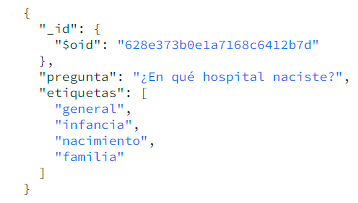
\includegraphics[scale=1.3]{Imagenes/Vectorial/mongo_pregunta}
	\caption{Documento de la colección de preguntas}
	\label{fig:mongo_preg}
\end{figure}

Por otro lado, la colección de respuestas contiene la información relativa a lo que ha respondido un usuario específico a una pregunta concreta. Es por eso, que el usuario que ha contestado y la pregunta respondida deben ser campos de esta colección. A continuación se explica cada uno de los campos:

\begin{itemize}
	\item ``user\_id'': Para distinguir al usuario se almacena el identificador que le corresponde una vez registrado en la página web. Los detalles de la aplicación web se explicarán en el capítulo siguiente. Sin embargo, para poder entender de dónde se extrae ese identificador, se explicará brevemente en que consiste. Diferentes usuarios pueden acceder al Chatbot desde la aplicación y para poder distinguir la información que se recopila es necesario tener un control de usuarios. Se crea una tabla en MySQL con todos los usuarios que se van registrando y a cada uno se le asigna un identificador. Este identificador es el que se va a guardar en la colección de respuestas para poder diferenciar las contestaciones que da cada usuario desde la página del Chatbot. En un principio, cuando la aplicación web no se había creado, no era necesaria la distinción de usuarios porque solo se invocaba al chatbot desde un único terminal asociado a una única persona. Es decir, las respuestas se podían almacenar suponiendo que siempre respondía la misma persona. No obstante, esta solución pierde escalabilidad. 
	\item ``pregunta'': Se corresponde con la pregunta que ha elegido el Chatbot para lanzar al usuario. Coincidiría con una de las muchas que están almacenadas en la colección de preguntas que se ha explicado anteriormente. 
	\item ``respuesta'': La contestación textual que ha dado el usuario a la pregunta formulada por el bot. 
	\item ``categorias'': Una serie de características que explican la respuesta. Entre ellas se encuentra la etapa de vida en la que puede encajarse el recuerdo y el resultado del análisis de sentimiento al que se le ha sometido en forma de ``positivo'' o ``negativo'' según las connotaciones reconocidas. Además, se almacenan los lemas extraídos mediante el procesamiento léxico que se ha explicado en la sección anterior. Se trata de los lemas de aquellas palabras del texto que no sean vacías y que definen a la contestación recibida. Se consigue un desglose y un análisis bastante exhaustivo de cada respuesta. 
\end{itemize}

En la figura \ref{fig:mongo_resp} se muestra un ejemplo de documento de la colección de respuestas.

\begin{figure}[h]
	\centering
	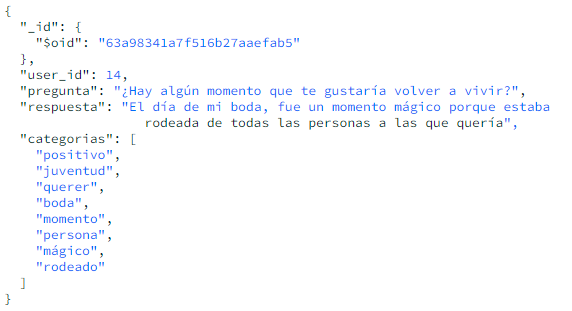
\includegraphics[scale=0.8]{Imagenes/Vectorial/mongo_respuesta}
	\caption{Documento de la colección de respuestas}
	\label{fig:mongo_resp}
\end{figure}


